%5_1.tex

実装した命令が正しく出力されるか,図\ref{fig:add_array_c}
に示した配列加算のプログラムを入力としてアセンブリコードの出力を行った.

\begin{figure}
    \centering
    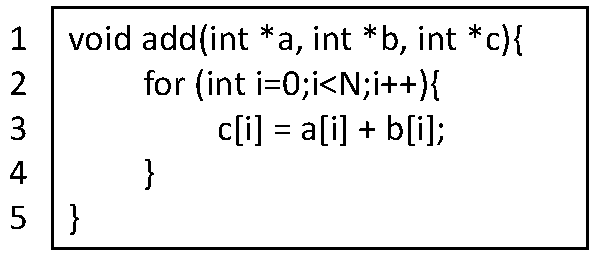
\includegraphics[scale=0.6]{image/add_array_c.pdf}
    \caption{配列加算プログラム}
    \label{fig:add_array_c}
\end{figure}

図\ref{fig:rv_vectorized_assembly}
配列a,bの各要素の加算を配列cに格納する関数addのアセンブリコードである.

\begin{figure}
    \centering
    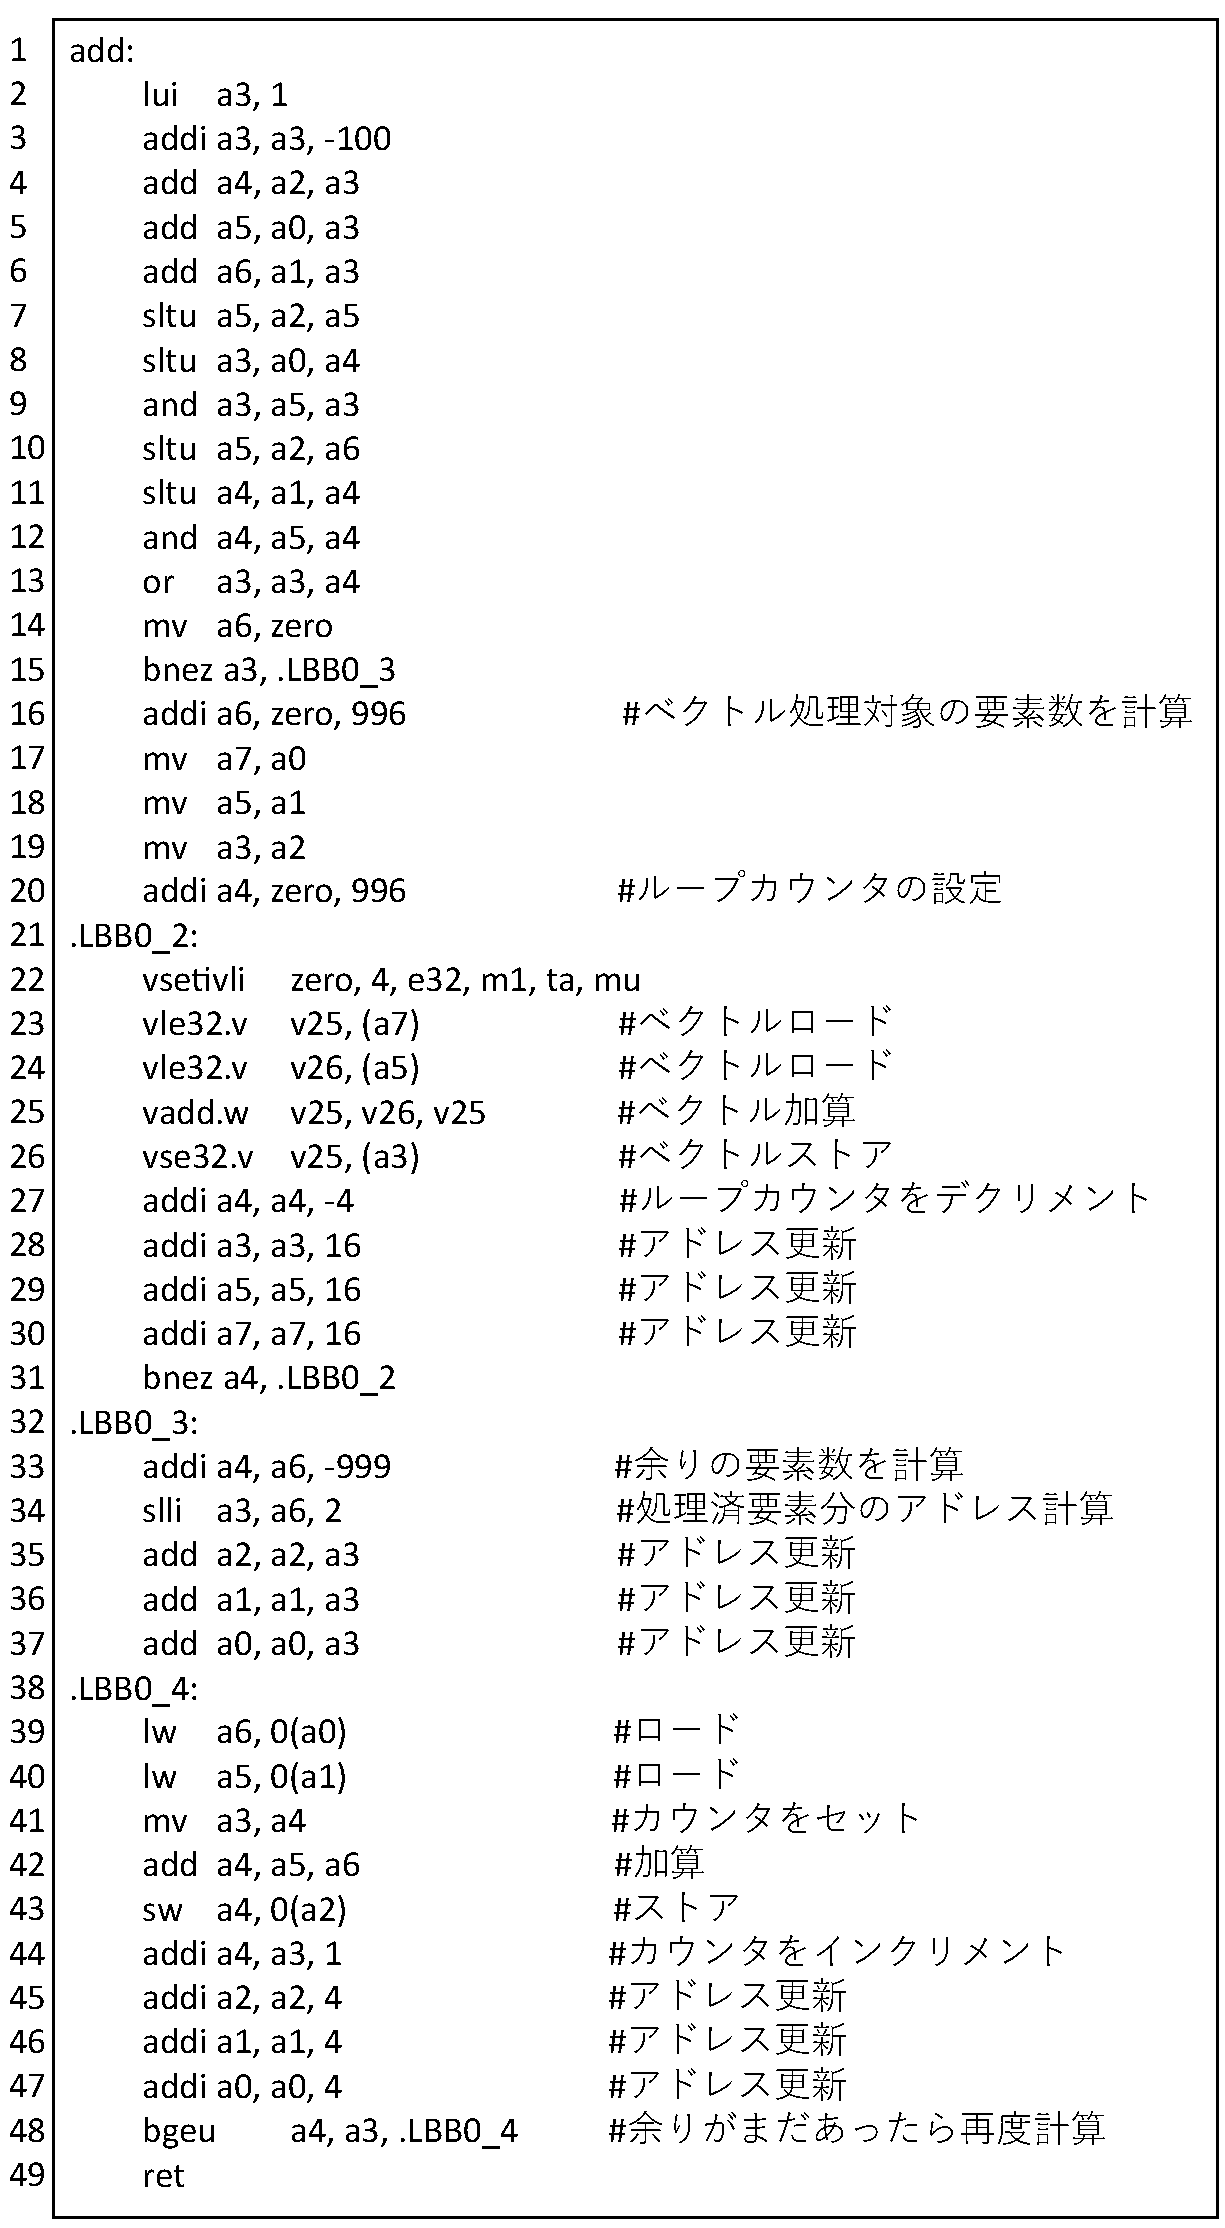
\includegraphics[scale=0.55]{image/rv_vectorized_assembly.pdf}
    \caption{生成されたアセンブリコード}
    \label{fig:rv_vectorized_assembly}
\end{figure}

